\chapter{Empirical Evaluation}
\label{chapter4}
We evaluate our various method implementations across a variety of domains. The goal of this evaluation is to discover how effectively our agents can explore and learn against other baseline methods. 
% The baseline methods that we consider are $\epsilon$-greedy and PRL. $\epsilon$-greedy was chosen as it is perhaps the most widely used random exploration strategy in practice. PRL is simply a naive model-based exploration method, that works in the same way as our method, except it is not equipped with the additional Meta Actions and was 
% chosen to evaluate the usefulness of the Meta Actions.
\section{Baselines}
In order to truly evaluate our framework implementations, we needed some baselines to compare against. Firstly, we chose $\epsilon$-greedy due to its ubiquity. Secondly, we chose "PRL", a model-based exploration method that always acts greedily with respect to current model, which is updated through observations; this is essentially our framework minus the Meta Actions. This was chosen as we wanted to evaluate the usefulness of Meta Actions. We decided not to compare against SOTA algorithms discussed in the literature review, as due to their complexities they would prove difficult to implement. Furthermore, it didn't seem like a fair comparison, as we made various simplifications when implementing our framework.
\section{Domains}
The domains that we chose to evaluate within were all gridworld-based. This decision was made due to the ease of modelling such domains, especially in a tabular manner. Furthermore, this enabled us to easily understand how the agents explore. Thus, the actions available to the agents are common between tasks (unless specified otherwise); up, down, left and right.
\\Gridworld is a deterministic domain, shown in Figure \ref{fig:domains}a. The agent starts in the middle of the room at the bottom of the grid. There are three doors to leave the room, in the left, right and top of the room. All of the doors are open, if they were closed then the agent would not know how to open them. The goal of the agent is to navigate to the other side of the top door. In our experiments, the model that the agents were seeded with indicated that the door leading to the goal was closed. The agent receives a reward of -1 at every time step.
\\Cliff-Walking \cite{Sutton1998} is a deterministic domain, shown in Figure \ref{fig:domains}b. The agent starts in the bottom left corner of the grid and needs to navigate to the goal state at the bottom right of the grid. However, there is a cliff along the bottom of the grid, which the agent needs to avoid. In our experiments, the model that the agents were seeded with indicated that the cliff was bigger than it actually is; it was along the bottom two rows of the grid. The agent receives a reward of -1 at every time step, unless it steps into the cliff which induces a reward of -100 and returns the agent to the start state (without terminating the episode).
\\Windy-Gridworld \cite{Sutton1998} is a deterministic domain, shown in Figure \ref{fig:domains}c. The agent starts in the left middle of the grid, and must navigate towards a goal state on the right-hand side of the grid. However, the is an upward wind within some columns which varies in strength. The wind shifts the next state upwards by the strength of the wind. In our experiments, the model that the agents were seeded with did not capture the wind. The agent receives a reward of -1 at every time step.
\\Stochastic Gridworld is the same as Gridworld, except there is some stochasticity introduced; the top door has a probability of 0.4 of being closed, within each episode. In our experiments, the model that the agents were seeded with indicated that the door leading to the goal was closed, with probability 1. The reward formulation and the actions available to the agent remain the same along with the seeded model.
\\Frozen Lake is a stochastic domain, shown in Figure \ref{fig:domains}d. The agent must navigate from the start state in the top-left corner to the goal state in the bottom-right corner. However, the frozen lake is slippery, meaning that the agent moves in the intended direction with probability $\frac{1}{3}$ and in either of the perpendicular directions with probability $\frac{1}{3}$ each. Furthermore, there are holes where the ice has been broken or melted and entering these holes terminate the episode. The model that the agents were seeded with did not capture the slipperiness of the frozen lake, and also suggests that there is only a single path to the goal state. Rewards are sparse; reaching the goal state returns a reward of +1, whilst at all other time steps the agent receives no reward.
\\Stochastic Windy-Gridworld is the same as Windy-Gridworld, except there is stochasticity introduced;  the wind (if there is any) is stochastic. The reward formulation and the actions available to the agent remain the same along with the seeded model.

% \begin{figure}[H]
%     \centering
%     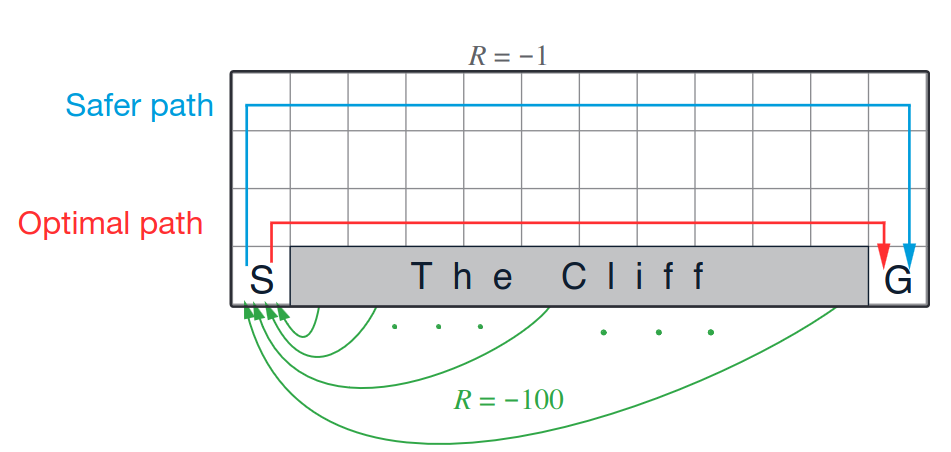
\includegraphics[max size={250}{250}]{report/assets/envs/cliff-walking.png}
%     \caption{Cliff-Walking Domain}
%     \label{fig:cliff_walking}
% \end{figure}

% \begin{figure}[H]
%     \centering
%     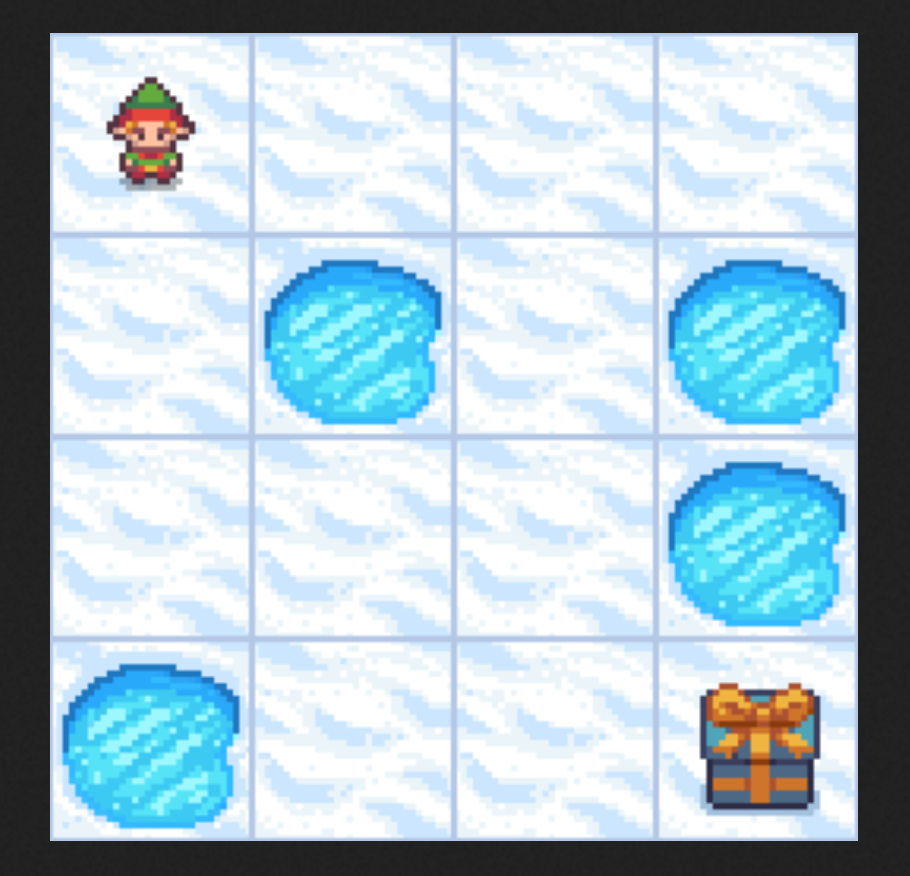
\includegraphics[max size={200}{200}]{report/assets/envs/frozen-lake.png}
%     \caption{Frozen Lake Domain}
%     \label{fig:frozen_lake}
% \end{figure}

\begin{figure}
\label{fig:domains}
\begin{tabular}{cc}
    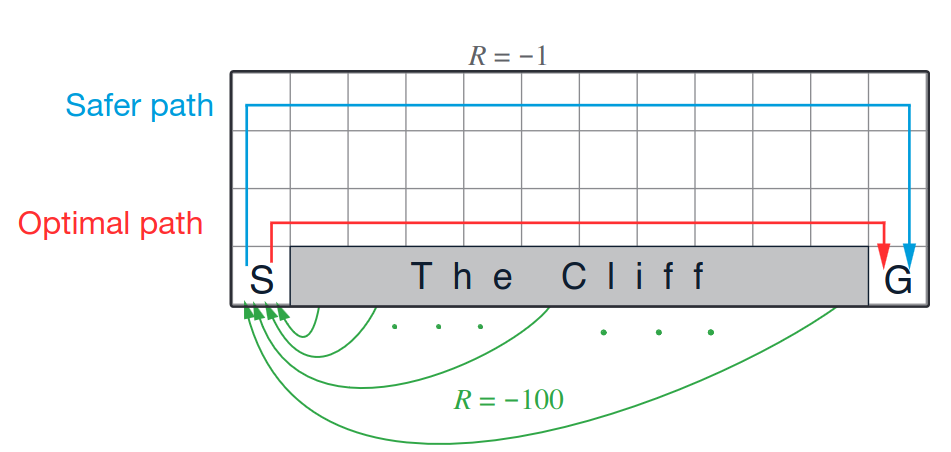
\includegraphics[width=65mm]{report/assets/envs/cliff-walking.png} & 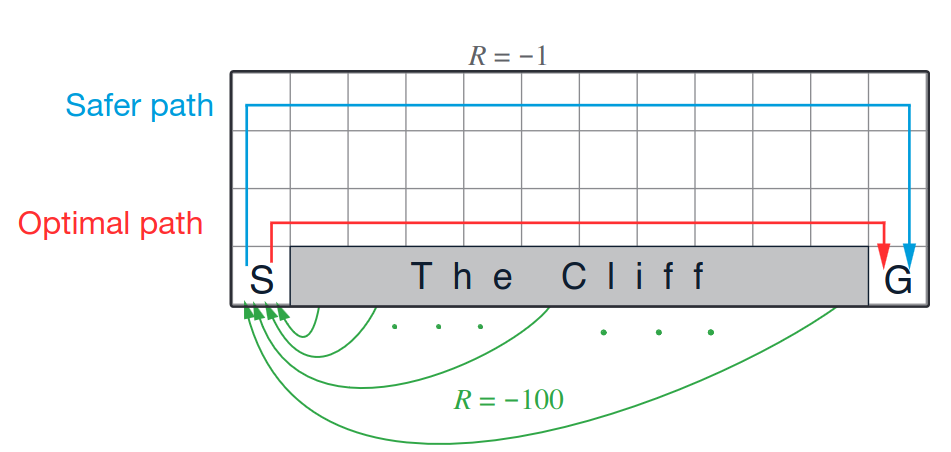
\includegraphics[width=65mm]{report/assets/envs/cliff-walking.png} \\
    (a) Gridworld & (b) Cliff Walking \\[6pt]
    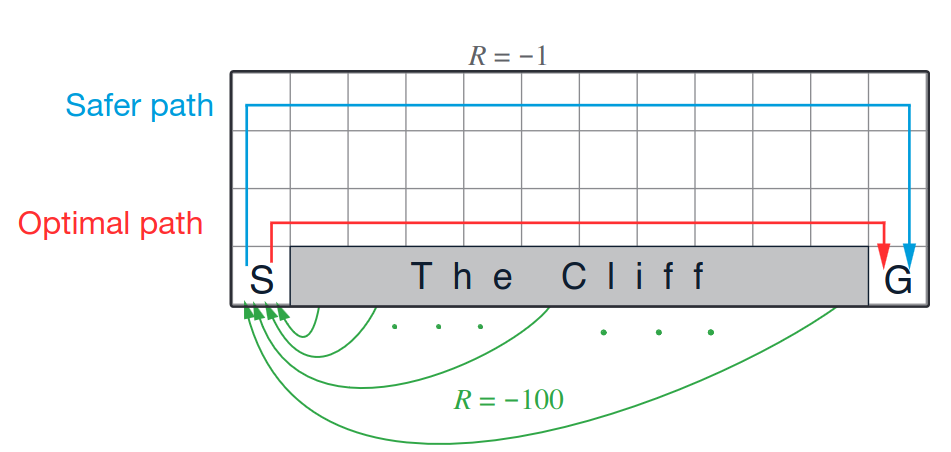
\includegraphics[width=65mm]{report/assets/envs/cliff-walking.png} & 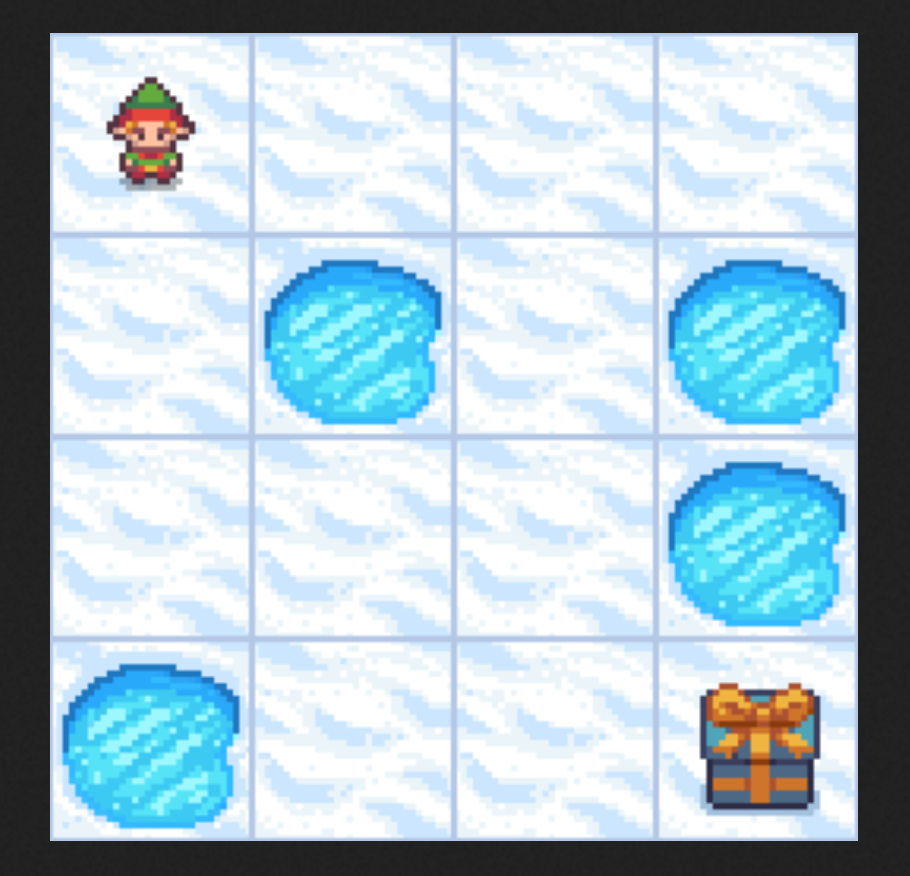
\includegraphics[width=65mm]{report/assets/envs/frozen-lake.png} \\[6pt]
    (c) Windy Gridworld & (d) Frozen Lake\\[6pt]
%   \includegraphics[width=65mm]{it} &   \includegraphics[width=65mm]{it} \\
% (a) first & (b) second \\[6pt]
%  \includegraphics[width=65mm]{it} &   \includegraphics[width=65mm]{it} \\
% (c) third & (d) fourth \\[6pt]
\multicolumn{2}{c}{\includegraphics[width=65mm]{it} }\\
\multicolumn{2}{c}{(e) fifth}
\end{tabular}
\caption{Domains}
\end{figure}

% The Frozen Lake domain \cite{1606.01540} is a stochastic gridworld, where the agent must navigate from the start state in the top left corner to the goal state in the bottom right corner, by using the actions "up", "down", "left" and "right". However, the frozen lake is slippery, meaning that the agent moves in the intended direction with probability $\frac{1}{3}$ and in either of the perpendicular directions with probability $\frac{1}{3}$ each. Furthermore, there are holes where the ice has been broken or melted and entering these holes end the epsisode. Rewards are sparse; reaching the goal state returns a reward of +1, whilst all other transitions return a reward of 0. The model that the model-based agents were seeded with did not model the slippery nature of the lake; thus the agents were unaware of it.

% The Cliff-Walking domain \cite{Sutton1998} is a deterministic gridworld, where the agent begins in the bottom left corner and needs to navigate to the goal state in the bottom right corner by using the actions "up", "down", "left" and "right". However, there is a cliff along the bottom of the grid. The goal of the agent is to reach the goal state whilst avoiding the cliff, as stepping into the cliff returns the agent to the start state (without ending the episode) and induces a large reward penalty of -100. All other transitions return a reward of -1. The model that the model-based agents were seeded with indicated that the cliff was bigger than it actually is; the cliff in the model took up the bottom two rows (minus the end states).

% The Windy Gridworld domain \cite{Sutton1998} is a deterministic gridworld, where the agent most navigate from the start state to the goal state, by using the actions "up", "down", "left" and "right". However, there is "wind" through the middle of the grid which varies in strength. The wind shifts the next state upwards by the strength of the wind. All transitions return a reward of -1. The model that the model-based agents were seeded with did not model the wind; thus the agents were unaware of it.



\section{Results}
\begin{figure}[H]
    \centering
    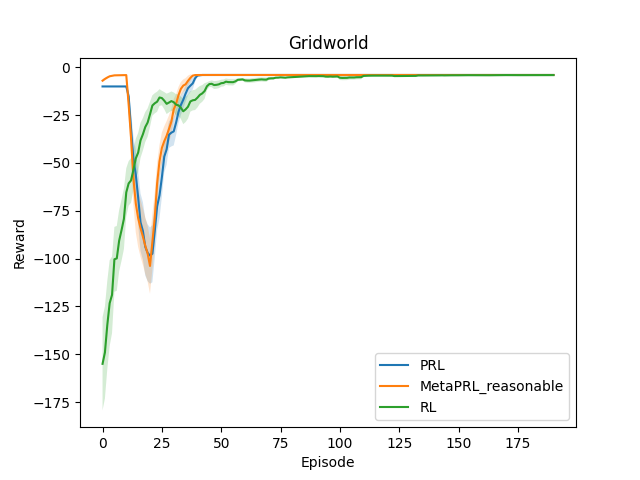
\includegraphics[max size={250}{250}]{report/assets/gridworld.png}
    \caption{Gridworld Results}
    \label{fig:deterministic_gridworld}
\end{figure}
\begin{table}[h]
\centering
\begin{tabular}{|c|c|c|c|c|c|}
\hline
\textbf{Agent} & \textbf{Min} & \textbf{Max} & \textbf{Mean} & \textbf{Std. Dev} & \textbf{Final}\\ \hline
\textbf{MetaPRL} & -104 & -4 & -10 & 19 & -4\\ \hline
\textbf{PRL} & -102 & -4 & -11 & 20 & -4\\ \hline
\textbf{RL} & -168 & -4 & -15 & 28 & -4 \\ \hline
\end{tabular}
\caption{Reward Summary for Gridworld}
\label{tab:example_table}
\end{table}
\begin{figure}[H]
    \centering
    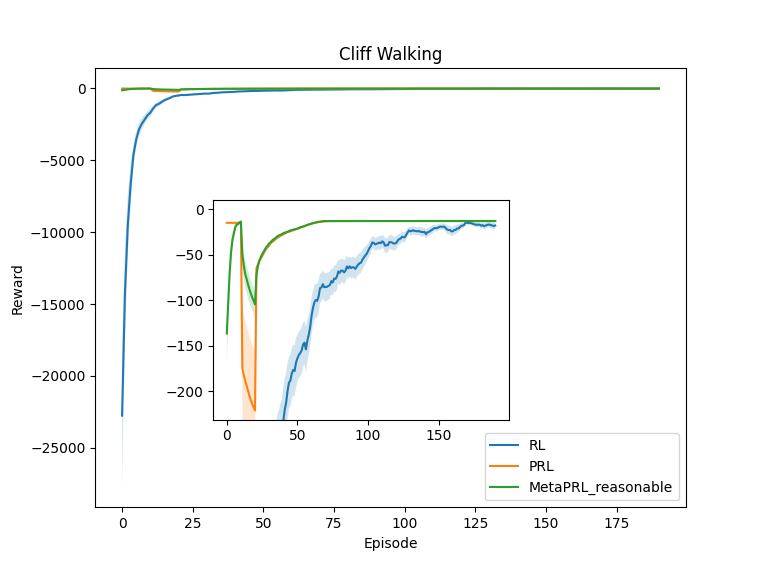
\includegraphics[max size={250}{250}]{report/assets/cliff_walking.png}
    \caption{Cliff-Walking Results}
    \label{fig:cliff_walking}
\end{figure}
\begin{table}[h]
\centering
\begin{tabular}{|c|c|c|c|c|c|}
\hline
\textbf{Agent} & \textbf{Min} & \textbf{Max} & \textbf{Mean} & \textbf{Std. Dev} & \textbf{Final}\\ \hline
\textbf{MetaPRL} & -137 & -13 & -22 & 21 & -13\\ \hline
\textbf{PRL} & -221 & -13 & -27 & 42 & -13\\ \hline
\textbf{RL} & -23099 & -14 & -520 & 2228 & -14 \\ \hline
\end{tabular}
\caption{Reward Summary for Cliff-Walking}
\label{tab:example_table}
\end{table}
\begin{figure}[H]
    \centering
    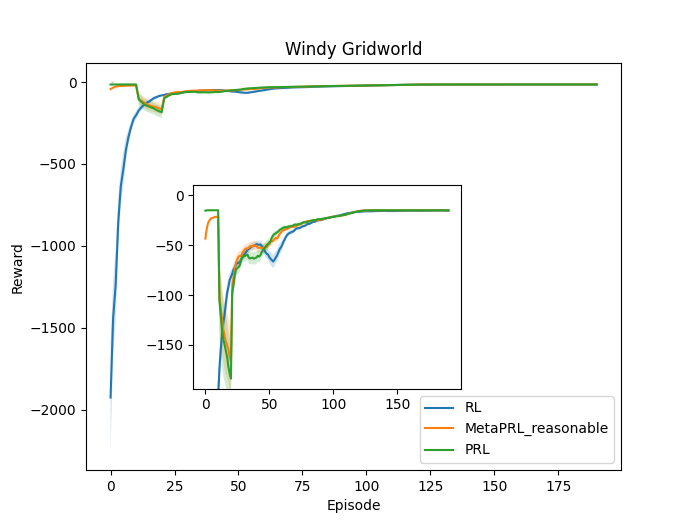
\includegraphics[max size={250}{250}]{report/assets/windy.png}
    \caption{Windy Gridworld Results}
    \label{fig:deterministic_wind}
\end{figure}

\begin{table}[h]
\centering
\begin{tabular}{|c|c|c|c|c|c|}
\hline
\textbf{Agent} & \textbf{Min} & \textbf{Max} & \textbf{Mean} & \textbf{Std. Dev} & \textbf{Final}\\ \hline
\textbf{MetaPRL} & -168 & -15 & -33 & 30 & -15\\ \hline
\textbf{PRL} & -183 & -15 & -34 & 33 & -15\\ \hline
\textbf{RL} & -2061 & -15 & -74 & 216 & -15 \\ \hline
\end{tabular}
\caption{Reward Summary for Windy Gridworld}
\label{tab:example_table}
\end{table}
\section{Analysis}
\begin{itemize}
    \item The dip.
    
\end{itemize}
% \begin{itemize}
%     \item State why we chose each domain, what we were evaluating, etc.
% \end{itemize}

% \section{Empirical Evaluation}
% We evaluated the performance of our agents within a range of domains, from self-designed domains to classic-control tasks. Most experiments were performed using OpenAI Gym \cite{1606.01540} and Behaviour Suite \cite{osband2020bsuite}. We organise the experiments into those that took place within deteriministic domains, and those which took place in stochastic domains. As baselines for evaluation, we used the PRL agent and $\epsilon$-greedy described in Chapter \ref{chapter2}. We chose the PRL agent, because we wanted to compare against a naive model-based exploration approach. Furthermore, we chose $\epsilon$-greedy as we wanted to compare to the most ubiquitous random exploration approach.
% \subsection{Deterministic Domains}
% \subsubsection{Gridworld}
% A deterministic gridworld, where the agent begins in the bottom middle, and needs to navigate to the goal state, using the actions "up", "down", "left" and "right". There is an open door, that if closed the agent wouldn't know how to open. All transitions return a reward of -1. The model that the model-based agents were seeded with indicated that the door was closed.





% \subsubsection{Cliff-Walking}
% The Cliff-Walking domain \cite{Sutton1998} is a deterministic gridworld, where the agent begins in the bottom left corner and needs to navigate to the goal state in the bottom right corner by using the actions "up", "down", "left" and "right". However, there is a cliff along the bottom of the grid. The goal of the agent is to reach the goal state whilst avoiding the cliff, as stepping into the cliff returns the agent to the start state (without ending the episode) and induces a large reward penalty of -100. All other transitions return a reward of -1. The model that the model-based agents were seeded with indicated that the cliff was bigger than it actually is; the cliff in the model took up the bottom two rows (minus the end states).

% % This domain can be seen in Figure \ref{fig:cliff_walking}.





% \subsubsection{Windy Gridworld}
% \label{sec:windy}
% The Windy Gridworld domain \cite{Sutton1998} is a deterministic gridworld, where the agent most navigate from the start state to the goal state, by using the actions "up", "down", "left" and "right". However, there is "wind" through the middle of the grid which varies in strength. The wind shifts the next state upwards by the strength of the wind. All transitions return a reward of -1. The model that the model-based agents were seeded with did not model the wind; thus the agents were unaware of it.




% \subsection{Stochastic Domains}
% \subsubsection{Stochastic Gridworld}
% A simple gridworld, with a door that is open with probability 0.5, closed otherwise. The model embedded suggests that the door is closed with probability 1.0.

% A stochastic gridworld, where the agent begins in the bottom middle, and needs to navigate to the goal state, using the actions "up", "down", "left" and "right". The door is open with probability 0.6 and closed otherwise. The agent does not have the ability to open the door. All transitions return a reward of -1. The model that the model-based agents were seeded with indicated that the door was closed with probability 1.0.

% \subsubsection{Stochastic Windy Gridworld}
% This is a stochastic version of the Windy Gridworld described in Section \ref{sec:windy}. The modification that makes it stochastic is that the wind (if there is any) is stochastic. Apart from that, the general setup is the same as previously described. Similarly, the model that the model-based agents were seeded with did not model the wind; thus the agents were unaware of it.

% %and seen in Figure \ref{fig:deterministic_wind}.

% \subsubsection{Frozen Lake}
% The Frozen Lake domain \cite{1606.01540} is a stochastic gridworld, where the agent must navigate from the start state in the top left corner to the goal state in the bottom right corner, by using the actions "up", "down", "left" and "right". However, the frozen lake is slippery, meaning that the agent moves in the intended direction with probability $\frac{1}{3}$ and in either of the perpendicular directions with probability $\frac{1}{3}$ each. Furthermore, there are holes where the ice has been broken or melted and entering these holes end the epsisode. Rewards are sparse; reaching the goal state returns a reward of +1, whilst all other transitions return a reward of 0. The model that the model-based agents were seeded with did not model the slippery nature of the lake; thus the agents were unaware of it.

% \section{An Ablation Study: Learning from Scratch}
% Within Chapter \ref{chapter2}, we stated that learning from scratch is a weakness of other model-based exploration approaches as models created by humans can be useful for learning. However, an interesting question is: is the usefulness of models created by humans worth the time it takes to construct them? This is what we investigate in this section. We seeded the various agents with optimistic initial models, as in the approach followed by R-MAX and OIM, however the so-called "Garden of Eden State" was a real-state in the environments, namely the actual goal state. Hence, the model suggests that every transition leads to the goal state.


% The ideas we have for future work mostly begin by solving the limitations outlined above. Most issues regarding scalability can be overcome by moving from exact to approximate solutions through function approximation methods; this would allow scaling to continuous, partially  observable domains. Furthermore, our method could be easily extended to domains with stochastic rewards, however in stateless domains such as Bandits, the criteria for calling a Meta Action that would increase reward needs to be further considered; this could be done by count-based methods or uncertainty based methods. Furthermore, more suitable planning algorithms could be explored, such as UCT \cite{10.1007/11871842_29}; which is the UCB algorithm \cite{auer2002finite} applied to tree search; this would offer a scalable, faster solution than Value Iteration. Consider generalization?
% \\Defining reasonability by known, unknown unvisited, similar to $E^3$, after the planning phase, don't visit any unvisited states?


% This domain can be seen in Figure \ref{fig:cliff_walking}.

% \begin{figure}[h!]
%     \centering
%     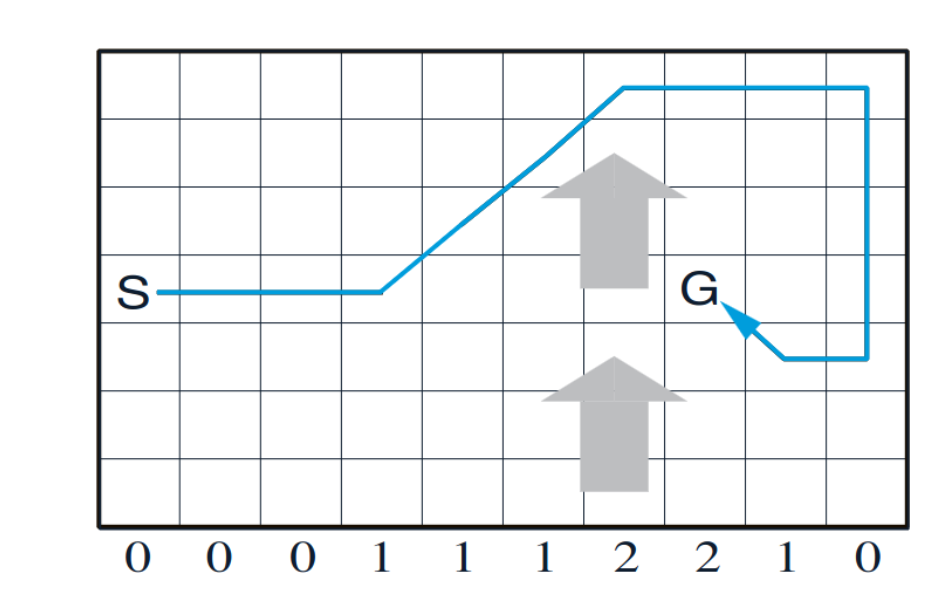
\includegraphics[max size={200}{200}]{report/assets/envs/windy.png}
%     \caption{Windy Gridworld}
%     \label{fig:deterministic_wind}
% \end{figure}


% \subsection{Cart-Pole}
% The Cart-Pole domain \cite{1606.01540, 6313077} consists of a pole placed on top of a moving cart, with the goal being to balance the pole by applying forces to the cart. There are two actions available to the agent; push cart left and push cart right. The agent's state is described by four variables; the cart's position, the cart's velocity, the pole's angle and the pole's angular velocity. 

% \begin{figure}[h!]
%     \centering
%     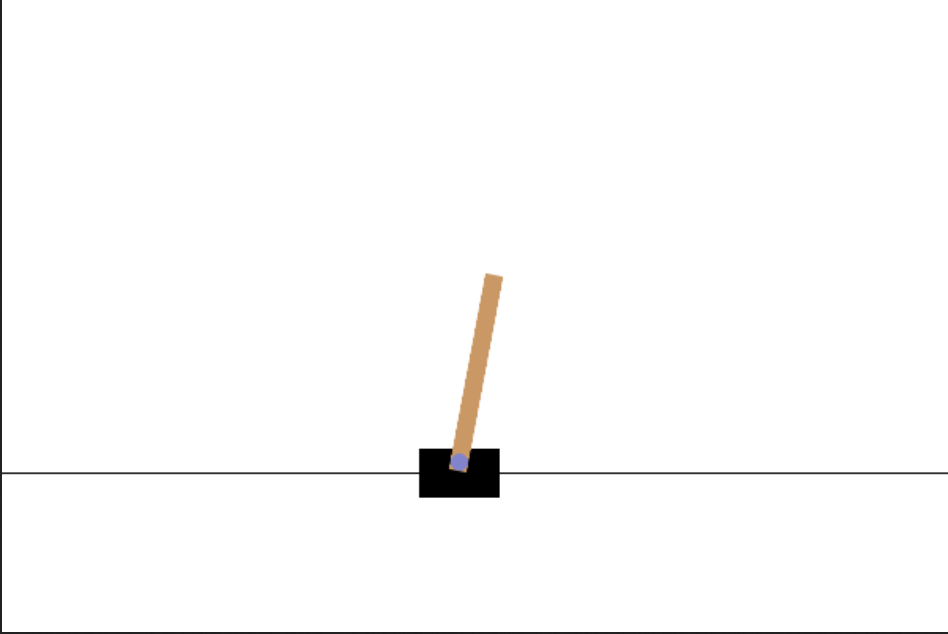
\includegraphics[max size={200}{200}]{report/assets/envs/cartpole.png}
%     \caption{Cartpole}
%     \label{fig:cartpole}
% \end{figure}


% \subsection{Mountain Car}
% The Mountain Car domain consists of a car placed stochastically in between two mountains, with the goal of getting to the top of the hill \cite{1606.01540, Moore90efficientmemory-based}. There are three actions available to the agent; accelerate left, don't accelerate and accelerate right. The agents state is described by two variables; it's velocity and it's position along the x-axis. 
% The transition function can be described by the following equations:
% \begin{equation}
% \label{eqn:mcdnl}
% \text{velocity}_{t+1} = \text{velocity}_t + (D * \text{F}) - \cos{(3*\text{position}_t)} * g
% \end{equation}
% \begin{equation}
% \label{eqn:mcdnr}
% \text{position}_{t+1} = \text{position}_t + \text{velocity}_{t+1}
% \end{equation}
% Where $D$ is the direction of acceleration: left = -1, none = 0, right = +1.
% All transitions return a reward of -1 and episodes are terminated after 200 time steps, if the goal has not been reached.


% \begin{figure}[h!]
%     \centering
%     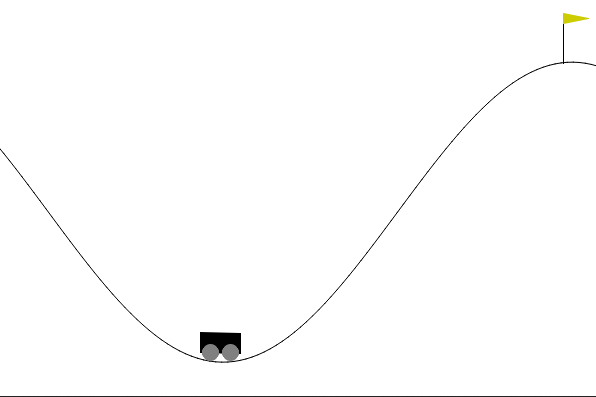
\includegraphics[max size={200}{200}]{report/assets/envs/mountaincar.png}
%     \caption{Mountain Car}
%     \label{fig:mountaincar}
% \end{figure}


% \section{Results}


% % This domain can be seen in Figure \ref{fig:frozen}

% \begin{figure}[h!]
%     \centering
%     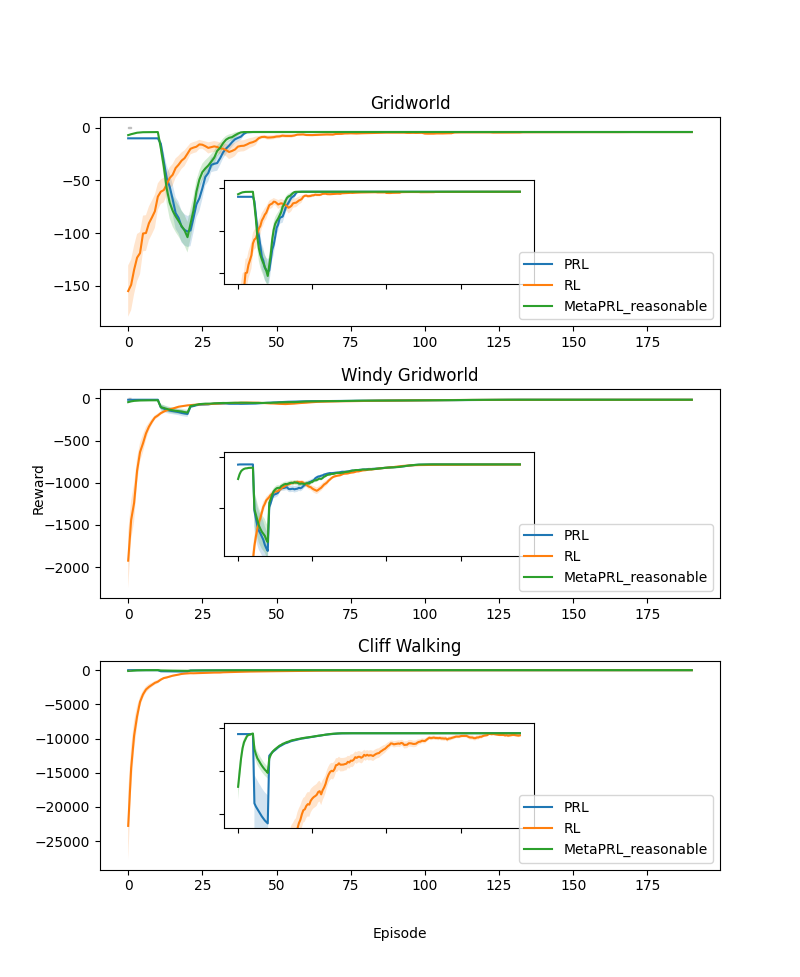
\includegraphics[max size={500}{500}]{report/assets/results.png}
%     \caption{Deterministic Results}
%     \label{fig:deterministic_results}
% \end{figure}